\documentclass[english,notitlepage,reprint]{revtex4-1}  % defines the basic parameters of the document

% if you want a single-column, remove reprint

% allows special characters (including æøå)
\usepackage[utf8]{inputenc}
\usepackage[english]{babel}

%% note that you may need to download some of these packages manually, it depends on your setup.
%% I recommend downloading TeXMaker, because it includes a large library of the most common packages.

\usepackage{physics,amssymb}  % mathematical symbols (physics imports amsmath)
\usepackage{graphicx}         % include graphics such as plots
\usepackage{xcolor}           % set colors
\usepackage{hyperref}         % automagic cross-referencing (this is GODLIKE)
\usepackage{tikz}             % draw figures manually
\usepackage{listings}         % display code
\usepackage{subfigure}        % imports a lot of cool and useful figure commands
\usepackage{lipsum}
\usepackage[ddmmyyyy]{datetime}
\usepackage{lmodern}

% (2) specify encoding
\usepackage[T1]{fontenc}
\usepackage{textcomp}
%\usepackage{unicode-math}
\usepackage{float}
\usepackage{balance}

% defines the color of hyperref objects
% Blending two colors:  blue!80!black  =  80% blue and 20% black
\hypersetup{ % this is just my personal choice, feel free to change things
    colorlinks,
    linkcolor={red!50!black},
    citecolor={blue!50!black},
    urlcolor={blue!80!black}}

%% Defines the style of the programming listing
%% This is actually my personal template, go ahead and change stuff if you want
\lstset{ %
	inputpath=,
	backgroundcolor=\color{white!88!black},
	basicstyle={\ttfamily\scriptsize},
	commentstyle=\color{magenta},
	language=Python,
	morekeywords={True,False},
	tabsize=4,
	stringstyle=\color{green!55!black},
	frame=single,
	keywordstyle=\color{blue},
	showstringspaces=false,
	columns=fullflexible,
	keepspaces=true}

\lstset{literate=
  {á}{{\'a}}1 {é}{{\'e}}1 {í}{{\'i}}1 {ó}{{\'o}}1 {ú}{{\'u}}1
  {Á}{{\'A}}1 {É}{{\'E}}1 {Í}{{\'I}}1 {Ó}{{\'O}}1 {Ú}{{\'U}}1
  {à}{{\`a}}1 {è}{{\`e}}1 {ì}{{\`i}}1 {ò}{{\`o}}1 {ù}{{\`u}}1
  {À}{{\`A}}1 {È}{{\'E}}1 {Ì}{{\`I}}1 {Ò}{{\`O}}1 {Ù}{{\`U}}1
  {ä}{{\"a}}1 {ë}{{\"e}}1 {ï}{{\"i}}1 {ö}{{\"o}}1 {ü}{{\"u}}1
  {Ä}{{\"A}}1 {Ë}{{\"E}}1 {Ï}{{\"I}}1 {Ö}{{\"O}}1 {Ü}{{\"U}}1
  {â}{{\^a}}1 {ê}{{\^e}}1 {î}{{\^i}}1 {ô}{{\^o}}1 {û}{{\^u}}1
  {Â}{{\^A}}1 {Ê}{{\^E}}1 {Î}{{\^I}}1 {Ô}{{\^O}}1 {Û}{{\^U}}1
  {œ}{{\oe}}1 {Œ}{{\OE}}1 {æ}{{\ae}}1 {Æ}{{\AE}}1 {ß}{{\ss}}1
  {ű}{{\H{u}}}1 {Ű}{{\H{U}}}1 {ő}{{\H{o}}}1 {Ő}{{\H{O}}}1
  {ç}{{\c c}}1 {Ç}{{\c C}}1 {ø}{{\o}}1 {å}{{\r a}}1 {Å}{{\r A}}1
  {€}{{\euro}}1 {£}{{\pounds}}1 {«}{{\guillemotleft}}1
  {»}{{\guillemotright}}1 {ñ}{{\~n}}1 {Ñ}{{\~N}}1 {¿}{{?`}}1
}

%% USEFUL LINKS:
%%
%%   UiO LaTeX guides:        https://www.mn.uio.no/ifi/tjenester/it/hjelp/latex/
%%   mathematics:             https://en.wikibooks.org/wiki/LaTeX/Mathematics

%%   PHYSICS !                https://mirror.hmc.edu/ctan/macros/latex/contrib/physics/physics.pdf

%%   the basics of Tikz:       https://en.wikibooks.org/wiki/LaTeX/PGF/TikZ
%%   all the colors!:          https://en.wikibooks.org/wiki/LaTeX/Colors
%%   how to draw tables:       https://en.wikibooks.org/wiki/LaTeX/Tables
%%   code listing styles:      https://en.wikibooks.org/wiki/LaTeX/Source_Code_Listings
%%   \includegraphics          https://en.wikibooks.org/wiki/LaTeX/Importing_Graphics
%%   learn more about figures  https://en.wikibooks.org/wiki/LaTeX/Floats,_Figures_and_Captions
%%   automagic bibliography:   https://en.wikibooks.org/wiki/LaTeX/Bibliography_Management  (this one is kinda difficult the first time)
%%   REVTeX Guide:             http://www.physics.csbsju.edu/370/papers/Journal_Style_Manuals/auguide4-1.pdf
%%
%%   (this document is of class "revtex4-1", the REVTeX Guide explains how the class works)


%% CREATING THE .pdf FILE USING LINUX IN THE TERMINAL
%%
%% [terminal]$ pdflatex template.tex
%%
%% Run the command twice, always.
%% If you want to use \footnote, you need to run these commands (IN THIS SPECIFIC ORDER)
%%
%% [terminal]$ pdflatex template.tex
%% [terminal]$ bibtex template
%% [terminal]$ pdflatex template.tex
%% [terminal]$ pdflatex template.tex
%%
%% Don't ask me why, I don't know.

\usepackage{thmtools}
\DeclareMathOperator{\nullspace}{Nul}
\DeclareMathOperator{\collspace}{Col}
\DeclareMathOperator{\rref}{Rref}
%%\DeclareMathOperator{\dim}{Dim}

 % "meq": must be equal
\newcommand{\meq}{\overset{!}{=}}

\newcommand{\R}{\mathbb{R}}
\newcommand*\Heq{\ensuremath{\overset{\kern2pt L'H}{=}}}
\usepackage{bm}
\newcommand{\uveci}{{\bm{\hat{\textnormal{\bfseries\i}}}}}
\newcommand{\uvecj}{{\bm{\hat{\textnormal{\bfseries\j}}}}}
\DeclareRobustCommand{\uvec}[1]{{%
  \ifcsname uvec#1\endcsname
     \csname uvec#1\endcsname
   \else
    \bm{\hat{\mathbf{#1}}}%
   \fi
}}
\usepackage{siunitx}

\makeatletter
\newcommand*{\balancecolsandclearpage}{%
  \close@column@grid
  \cleardoublepage
  \twocolumngrid
}
\makeatother

\newcounter{subproject}
\renewcommand{\thesubproject}{\alph{subproject}}
\newenvironment{subproj}{
\begin{description}
	\item[\refstepcounter{subproject}(\thesubproject)]
}{\end{description}}


\begin{document}
\title{Project 1 FYS3150}   % self-explanatory
\author{Anders P. Åsbø, Eivind Støland}               % self-explanatory

%\date{\today}
\noaffiliation                            % ignore this

\maketitle
\tableofcontents

\section{Introduction} \label{sec:I}
One of the most versitile tools in modern science is numerical integration, thus it it simportant to understand its limits. In this paper we have performed numerial integration of a second order differential equation. This was done by discretizing the differential equation, and formulating it as a matrix-vector equation. The matrix-vector equation was then solved using both a general, and specialzed Thomas algorithm, as well as LU-decomposition. Under the pretext of solving a \(1\)D version of Poisson's equation, we have created and tested a numerical solver using the Thomas algorithm. Furthermore, we have compared our results with LU decomposition using the Armadillo librarys solver.

\section{Formalism} \label{sec:II}


\section{Implementation} \label{sec:III}

\section{Analysis} \label{sec:IV}
\subsection{Plots of the general Thomas algorithm} \label{subsec:IV:A}
\begin{figure}[H]
	\centering
	\label{fig:iv:a:1}
	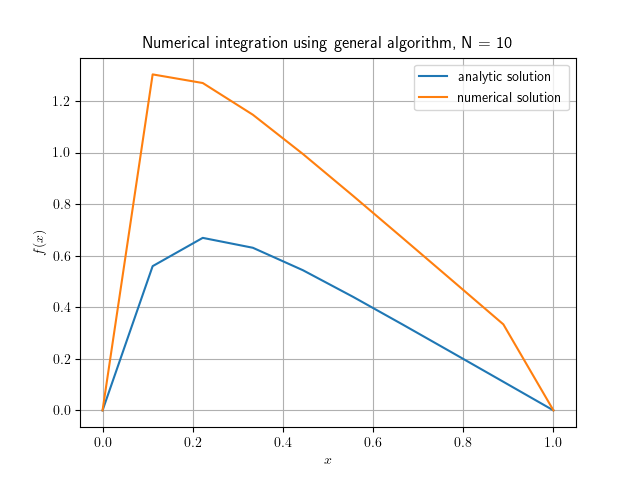
\includegraphics[width=\columnwidth]{plots/Figure_1.png}
	\caption{Plot of numerical and analytical solution, using the general Thomas algorithm with
	\(N=10^{1}\).}
\end{figure}

\begin{figure}[H]
	\centering
	\label{fig:iv:a:2}
	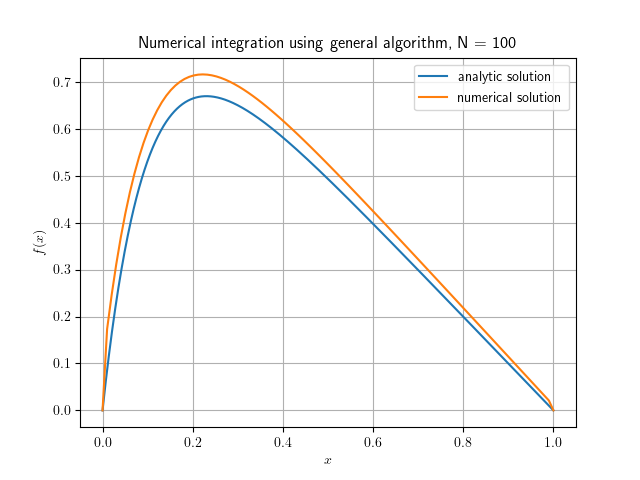
\includegraphics[width=\columnwidth]{plots/Figure_2.png}
	\caption{Plot of numerical and analytical solution, using the general Thomas algorithm with
	\(N=10^{2}\).}
\end{figure}

\begin{figure}[H]
	\centering
	\label{fig:iv:a:3}
	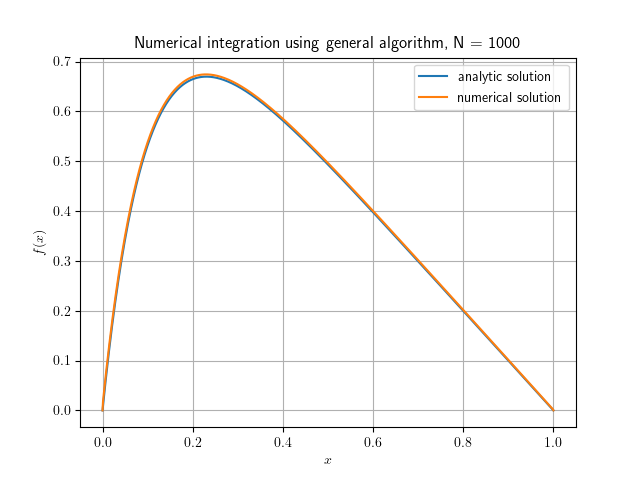
\includegraphics[width=\columnwidth]{plots/Figure_3.png}
	\caption{Plot of numerical and analytical solution, using the general Thomas algorithm with
	\(N=10^{3}\).}
\end{figure}

\subsection{Relative error for Thomas' algorithms} \label{subsec:IV:B}
\begin{table}[H]
	\label{table:iv:a:1}
	\begin{tabular}{|c|c|c|c|}
		\(\log_{10}(h)\): & \(\epsilon\) general algorithm & \(\epsilon\) special algorithm & \(N\) \\
		\(\num{-1.041393e+00}\) & \(\num{3.026200e-01}\) & \(\num{3.601314e-01}\) & \(10^{1}\) \\
		\(\num{-2.004321e+00}\) & \(\num{3.426303e-02}\) & \(\num{4.249885e-02}\) & \(10^{2}\) \\
		\(\num{-3.000434e+00}\) & \(\num{3.474750e-03}\) & \(\num{4.338587e-03}\) & \(10^{3}\) \\
		\(\num{-4.000043e+00}\) & \(\num{3.479720e-04}\) & \(\num{4.347831e-04}\) & \(10^{4}\) \\
		\(\num{-5.000004e+00}\) & \(\num{3.480179e-05}\) & \(\num{4.348760e-05}\) & \(10^{5}\) \\
		\(\num{-6.000000e+00}\) & \(\num{4.210129e-06}\) & \(\num{4.348746e-06}\) & \(10^{6}\) \\
		\(\num{-7.000000e+00}\) & \(\num{1.005169e-06}\) & \(\num{4.343971e-07}\) & \(10^{7}\) \\
		\(\num{-8.000000e+00}\) & \(\num{-1.140500e-03}\) & \(\num{3.765295e-08}\) & \(10^{8}\)
	\end{tabular}
	\caption{Table with \(\log_{10}\) of relative error for general and special Thomas' algorithms, and \(\log_{10}\) of step size \(h\)}
\end{table}

\section{Conclusion} \label{sec:V}

\bibliography{kilder}{}

\appendix
\section{Source code}
All code for this report was written in C++ and Python 3.8, and the complete set of files can be found at \url{https://github.com/FunkMarvel/FYS3150_Project_1.git}

\end{document}
